\documentclass{article}
\usepackage[utf8]{inputenc}
\usepackage{float}

\title{\textbf{Preliminary Research Proposal}\\Investigating the Microscopic Mechanics of Hair-Hydrometer via Atomic Force Microscopy }
\author{Jun-Yan Zhang, Yue-Jian Mo}

\date{August 2019}

\usepackage{natbib}
\usepackage{graphicx}

\begin{document}

\maketitle

\begin{abstract}
    
\end{abstract}

\section{The Problem}
\begin{itemize}
\item What's the microscopic mechanism of the Hair-Hydrometer?
\item How a normal kerotin in human hair change in morphology and its Young's Modulus with the change of environment humidity and temperature? 
\item What's the relationship between the kerotin's mechanical properties and the macroscopic mechanical properties of human hair?
\end{itemize}

\section{Background}
A simple hygrometer can be built stretching a bunch of degreased human hair, invented in 1800 by a swiss physicist and the founder of mountaineering, de Saussure. Even now the hair-hydrometer is still playing an important role in meteorological oservatories all over the world because its high precision. \\
The stiffness of the hair will change with the humidity, temperature and other factors of the environment and thus the hair length will change under a fixed tension applied at two endings of the hair. The previous work done by our team found out the rough relation between hair length and environment factors in a macroscopic view, and we hypothised a physical model to explain the phenomenon using estimated density of Hydrogen bonds between kerotins, which is the core compounds consisting human hair and the chemical equilibrium of Hydrogen bond breaking under different humidity and temperature (hydrogen bonds provide a part of the hair's stiffness), but the microscopic mechanics is still under debating.

Enlightened by the Atomic Force Microscopic(AFM) imaging for Young's Modulus(YM) of amyloid fibrils \citep{lee2016advances}(they used an advanced AFM mode, Peak Force Quantitative Nanomechanics Measurement (Peak Force QNM) mode, to get the \textbf{radial} YM data of amyloid fibrils under different conditions (e.g., in different environment, after different incubation time) by nano-indentation), we came up an idea that to make kerotins fibrils as the specimen instead of amyloid fibrils.  \\
We can control the environment easily by setting up the whole instrument in a artificial box allowing us to adjust the humidity and the temperature.

\subsection{Literature review}
At beginning (1921), people thought it was humidity that changes the curvature of water menisci in the hair cell pores and then strain or loosen the cell walls. The mechanical properties of hair follows Hooke's law\citep{Whipple_1921}.
\begin{figure}[H]
    \centering
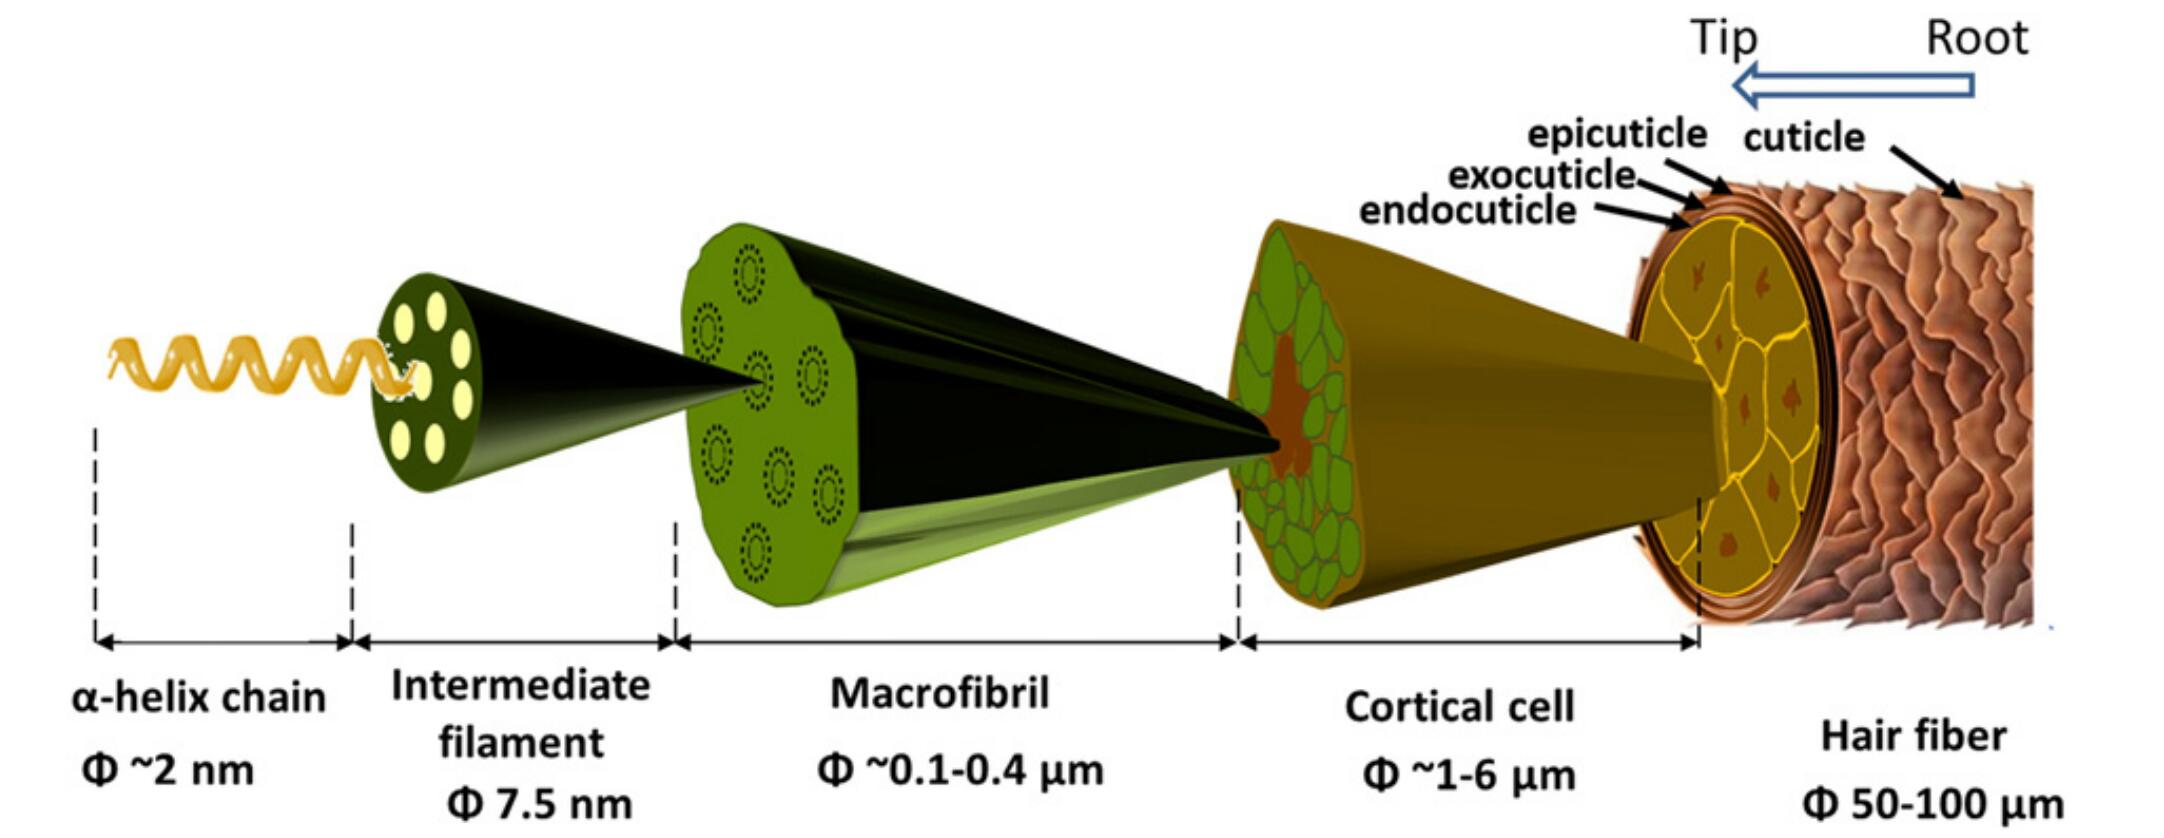
\includegraphics[width=0.8\textwidth]{hair structure.jpg}
    \caption{hair structure\citep{yu2017structure}}
    \label{hair structure}
\end{figure}
Human Hair is mainly consisted by curtail, cortex, and medulla from outside to the center. In one paper, they used $\alpha$ and $\beta$ kerotin model (examined by X-ray scattering) to explain the elasticity of human hair:
\begin{figure}[H]
    \centering
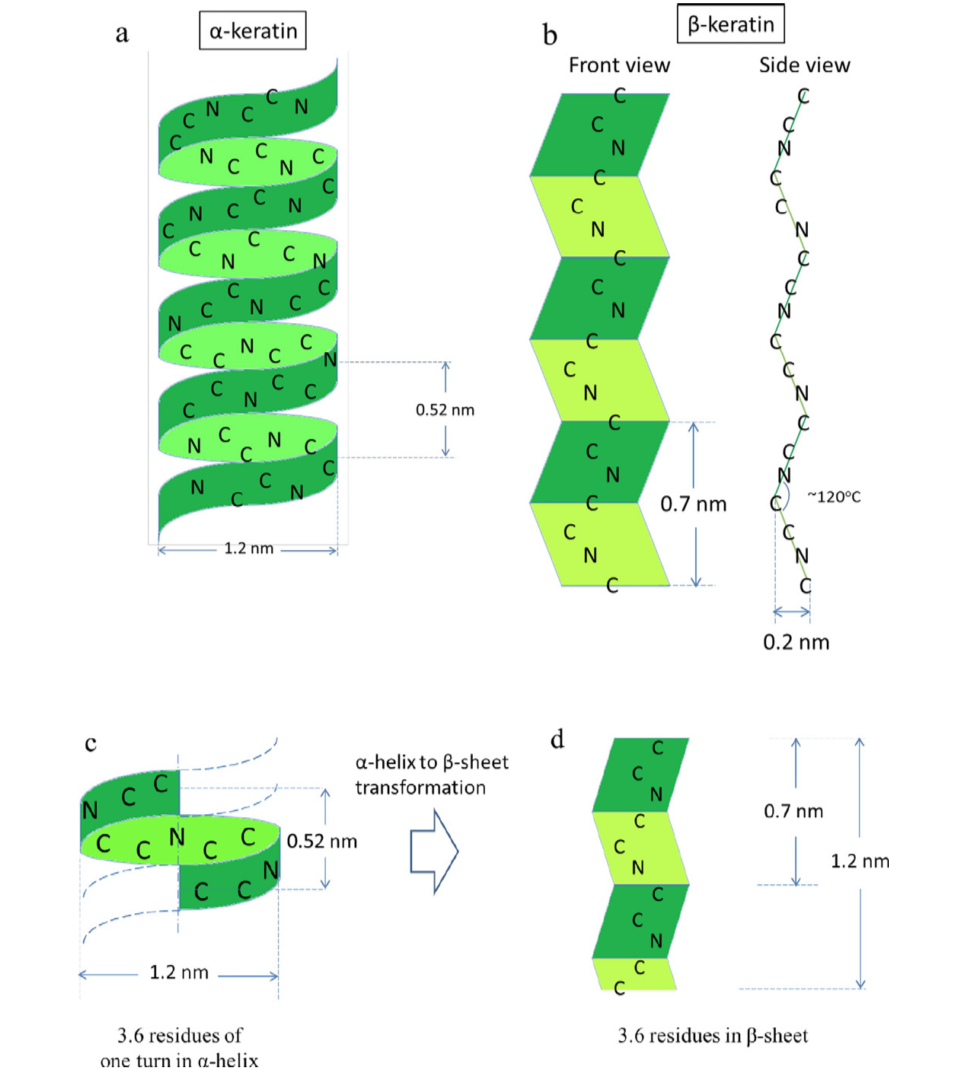
\includegraphics[width=0.6\textwidth]{protein structure.png}
    \caption{protein structure\citep{yu2017structure}}
    \label{protein structure}
\end{figure}
but they didn't consider the humidity acting on the chemical bond inside keratin.

Many AFM studies on nanomechanical properties of human hair(mainly on cellular structure) was done by Bhushan in Ohio State University\citep{bhushan2006afm}. But this work is not about the keratin and they mapped only lateral not longitudinal. 
\begin{figure}[H]
    \centering
    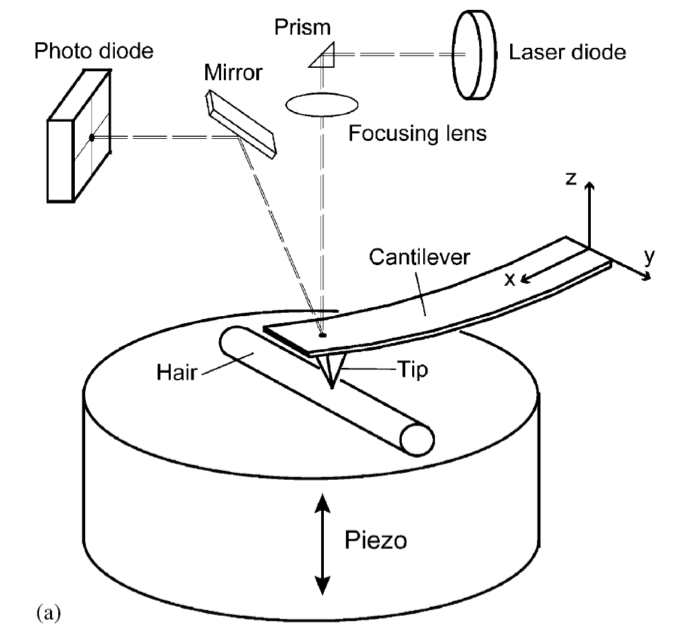
\includegraphics[width=0.4\textwidth]{bhushan.png}
    \caption{Bhushan's method}
\end{figure}

Simulation and mesoscopic experiments are done in \citep{}

Since there are numerous physical models and explanations, the first thing to do is focusing on the second problem. Then we can develop the solution to the third and the first, which is the core.


\section{Design}
\subsection{Modeling}
\begin{itemize}
    \item 
\end{itemize}

\subsection{Instrumentation}
\textbf{Specimen}: different kerotin fibrils, hairs\\ 
\textbf{AFM}: AFM, T-shaped cantilever with normal tip, oblong cantilever\\
Environment control: Humidity\&Temperature control box (using raspberry and electronic hydrometer\&thermometer to feedback), covering the whole AFM head.

\subsection{Method}
First, we measure the keratin protein's YM under different humidity and temperature. Second, measure how keratin effect hair's YM (i.e. by control variables only related to keratin inside hair, like using special enzyme(keratinase\citep{lin1992purification}) solution which can influent keratin to process the hair).  Third, set up the keratin-hair mechanical model, comparing to known model and do the simulation.


\textbf{Notice}: we need to bias the humidity influence on adhesion between tip and specimen.

\subsection{Difficulties}
\begin{itemize}
    \item How to measure the axial Young's modulus of a nano fiber? and How to fix an end of kerotin fibrils?
    
    \item How to develop a better hair mechanical model? There must be other relevant factors.

	\item How to control variates? like How to only destroying the protein fibrils inside the hair?
\end{itemize}


\section{Expected Result}
Expected to have 
\begin{itemize}
	
	\item a decreased keroin YM with increasing humidity and temparature.
	 \item a proportional relationship between kerotin fibrils YM and hair YM (longitudinal). 
\end{itemize}
\subsection{Expected Finishing Time}

\bibliographystyle{plain}
\bibliography{references}
\end{document}



